\documentclass[12pt]{article}

% Science format fonts
\usepackage{newtxtext,newtxmath}

% Page layout
\usepackage[margin=1in]{geometry}

% Allow external graphics
\usepackage{graphicx}

% Math support
\usepackage{amsmath}

% Figure and Table labels in bold
\makeatletter
\renewcommand{\fnum@figure}{\textbf{Fig.\ \thefigure}}
\renewcommand{\fnum@table}{\textbf{Table \thetable}}
\makeatother

% Reference section heading
\renewcommand\refname{References and Notes}

% Double line spacing, including in captions
\linespread{2.0}

% One space after each sentence
\frenchspacing

% Abstract formatting and spacing - no heading
\renewenvironment{abstract}
	{\quotation}
	{\endquotation}

% No date in the title section
\date{}

% Citation style
\usepackage{scicite}

% URL support
\usepackage{url}
\def\UrlBreaks{\do\/\do-\do.\do_\do~}

%%%%%%%%%%%%%%%% TITLE AND AUTHORS %%%%%%%%%%%%%%%%

\def\scititle{The Geography of Nobel Prize Selection}
\title{\bfseries \boldmath \scititle}

% One-sentence summary (for submission metadata, <= 125 characters):
% Geographic concentration in Nobel Prize selection is localized at the nomination decision, not institutional design.

\author{%
Chad M.\ Topaz$^{1,2,3,\ast}$,
Anvi Kurongonayini$^{2}$,
Bennett Ptak$^{2}$,
Arden Fluehr$^{2}$,\\
Ariana Mendible$^{4}$,
Rachel Roca$^{5}$,
Nancy Rodr\'{i}guez$^{3}$,
Lu Xian$^{6}$,
R\'{e}gan Schwartz$^{2}$,\\
Jude Higdon$^{1,7}$\\[10pt]
\normalsize $^{1}$QSIDE Institute.
$^{2}$Williams College.
$^{3}$University of Colorado--Boulder.\\
\normalsize $^{4}$Seattle University.
$^{5}$Michigan State University.
$^{6}$University of Michigan.\\
\normalsize $^{7}$Bennington College.\\[4pt]
\small $^\ast$Corresponding author. Email: cmt6@williams.edu
}

%%%%%%%%%%%%%%%% START OF MAIN TEXT %%%%%%%%%%%%%%%

\begin{document}

\maketitle

\begin{abstract}
Five countries account for over 80\% of Nobel Prize--winning discoveries. Because high-prestige recognition redirects resources and talent, such concentration can be self-reinforcing, yet whether it originates in institutional design or individual evaluator behavior is unknown. We decomposed Nobel selection into a five-layer network spanning 8,134 individuals, 514,111 edges, and five prize categories (1901--1975). The Swedish and Norwegian bodies that oversee Nobel selection assembled a geographically diverse nominator pool, yet within it, nominators select same-country nominees 4.85 times as often as expected ($p < 0.001$), from 8.58$\times$ in Literature to 3.01$\times$ in Physics. This concentration persisted as the nominee pool diversified over seven decades. Geographic sorting enters at the discretionary nomination decision, not the institutional pipeline---a specific, targetable point in the selection process.
\end{abstract}

\noindent The Nobel Prize is the most prestigious international prize \cite{CasFan2013}. Scientists from Europe or North America have received the vast majority of these prizes \cite{LunJenJau2019, ChaEllRah2011, Cra2001}, and just five countries account for over 80\% of prize-winning discoveries \cite{vonZed2025}. Geographic concentration reinforces cumulative advantage: regions whose scientists receive prizes attract disproportionate funding, talent, and further recognition \cite{Mer1968, Zuc1977, ColCol1973, Gar1972}, creating a feedback loop in which the geography of past recognition shapes the geography of future scientific capacity. Within prize-winning countries, racial and ethnic disparities further narrow who receives recognition \cite{NeiVueVue2024}. Whether these disparities arise from how candidates are selected or from where scientific output is produced remains unclear, yet this distinction determines the appropriate reform: if concentration were primarily institutional, diversifying committee membership would be the natural intervention, but if it arises at the nomination stage, reform must instead target the thousands of individual evaluators whose choices collectively shape the candidate pool. Homophily, the tendency for similar individuals to form ties \cite{McPSmoCoo2001}, offers a way to localize where geographic sorting enters: comparing observed same-geography rates to expected rates at each stage of a selection chain can identify the decision point at which concentration appears.

The architecture of the Nobel system offers an opportunity to localize this sorting. Each prize has a \emph{governing body} that oversees the process: the Royal Swedish Academy of Sciences (RSAS) for Chemistry and Physics, the Nobel Assembly at the Karolinska Institutet for Physiology or Medicine, the Swedish Academy for Literature, and the Storting (Norwegian parliament) for Peace. The governing body appoints a \emph{vetting body}, a Nobel Committee of roughly five members, that solicits nominations, commissions expert evaluations, and recommends finalists. \emph{Nominators} submit candidates: for three prizes they participate by invitation only, while for Literature and Peace any eligible individual may nominate. The governing body makes the final selection of laureates, except for Peace, where the Nobel Committee itself decides \cite{methods}. Each of these layers could introduce or amplify geographic concentration. Prior work shows that Nobel nominations cluster by country \cite{GalDom2019} and that laureates occupy central positions in collaborative networks \cite{WagHorWhe2015}. Beyond the Nobel context, same-country reviewers of scientific journal manuscripts recommend acceptance more often \cite{ZumTep2025}. Gendered barriers further constrain who enters the nomination pipeline \cite{ModGilSha2018, LunJenJau2019}. But single-layer analyses of the nominator--nominee relationship \cite{GalDom2019} cannot determine whether observed clustering reflects nominator preferences or the committees' selection of nominators---if the all-Scandinavian committees disproportionately invited nominators from a narrow set of countries, the resulting nominations would cluster by country even without nominators' individual geographic preference. Regression-based approaches \cite{KoJanYan2024} face a similar identification problem.

We address this gap by decomposing the selection process into a multilayer network \cite{Kivela2014} with separate edge sets for each decision point. If the all-Scandinavian committees were the primary source of geographic sorting, we would expect a geographically skewed nominator pool: committees disproportionately inviting Scandinavian nominators. If nominators were the primary source, we would expect a diverse nominator pool, but a concentration in the nominations those individuals make. We assess which pattern the data support by comparing the geographic composition of each layer and computing homophily ratios for each edge type.

\subsection*{Network Construction and Homophily Measurement}

We constructed a directed multilayer network spanning all five original Nobel Prize categories---Chemistry, Physics, Physiology/Medicine, Literature, and Peace---from 1901 to 1975, the most recent publicly available years under Sweden's 50-year secrecy rule (Fig.~\ref{fig:schematic}). We excluded the Economics Prize, established in 1969, because of its different institutional structure and limited archival overlap. The network has five layers: governing bodies, vetting bodies, nominators, nominees, and laureates. We refer to governing bodies and vetting bodies as institutional layers. Temporal coverage varies by prize: Physiology/Medicine nomination records extend only through 1953 because its governing body has not released later records; institutional-layer data extend through the present. We identified each individual's country using two sources: for nominators and nominees, the country of professional activity recorded in the nomination archive; for institutional layers, the birth country from Wikidata, a structured biographical database. The two definitions differ because the nomination archive records professional affiliation at the time of each nomination, while institutional-layer members lack equivalent professional-country records; a robustness check using birth country throughout confirms our core finding \cite{methods}.

No prior dataset integrates all five layers of Nobel selection. We assembled the network by scraping, reconciling, and entity-resolving over ten distinct sources---including parliamentary rosters, digitized state calendars, the Nobel Prize Nomination Archive, and structured biographical databases---into a single graph of 8,134 individuals from over 100 modern countries and 514,111 directed edges: 26,654 nominations and 487,457 institutional edges \cite{methods}.
We modeled relationships among the five layers as complete bipartite connections, linking every member of one body to every member of the next, within each year and prize category, reflecting their collective nature. This construction means that network-level homophily ratios primarily reflect the composition of the network rather than preferences for same-group connections, a point we return to below. 

To measure geographic sorting, we computed a homophily ratio $H = O/E$ for each edge type at three scales: country, subregion---geographic clusters such as Northern Europe and Eastern Asia---and continent. The ratio divides the observed fraction of same-geography edges ($O$) by the fraction expected under random pairing ($E$). A ratio of 1.0 indicates geographic neutrality; values above 1.0 indicate concentration. We assessed significance with 10,000-fold permutation tests that shuffle target geographies while holding source geographies fixed, preserving the marginal distributions \cite{methods}. As a complementary measure, we report Newman assortativity $r$ \cite{New2003}, a correlation-like index of geographic mixing that ranges from $-1$ to $1$, with higher values indicating stronger sorting. Stratified analyses by discipline and decade, along with full construction details, subregion definitions, and sensitivity checks, appear in \cite{methods}.

\subsection*{Homophily Concentrates at the Nomination Edge}

The governing and vetting bodies were nearly entirely European (97.6\% and 98.9\%), with 84.7\% and 96.3\% of their members born in Sweden, Norway, or Denmark, while the nominator, nominee, and laureate layers were more diverse, at 65.7--71.3\% European. The effective number of subregions---the equivalent number of equally represented subregions, based on Shannon entropy \cite{methods}---was 6.30 for nominators, 5.80 for nominees, and 5.97 for laureates, versus 1.23--1.65 for institutional layers. Despite this compositional contrast, geographic homophily concentrated in a single edge type: the nominator $\to$ nominee relationship (Fig.~\ref{fig:edge_homophily}).

At the country level, the nominator $\to$ nominee homophily ratio was 4.85 ($p < 0.001$, permutation test against geographic neutrality): nominators and their nominees shared a country nearly five times more often than expected (observed same-country rate 46.8\%, versus 9.6\% expected; 25,844 edges; Fig.~\ref{fig:edge_homophily}). For context, geographic homophily in social networks is pervasive but typically moderate \cite{McPSmoCoo2001}, and same-country peer reviewers recommend acceptance at only moderately elevated rates \cite{ZumTep2025}; a ratio of 4.85 indicates exceptionally strong clustering. This finding is robust to alternative geographic definitions (birth country yields $H = 3.82$, $p < 0.001$), blockwise permutations within prize-year strata, Bonferroni correction across 49 tests, and clustered permutations preserving within-nominator correlation \cite{methods}.

To isolate where geographic sorting entered the selection pipeline, we first examined the institutional edges. The governing body $\to$ laureate, vetting body $\to$ nominator, and vetting body $\to$ laureate edges all showed homophily ratios near 1.0 at the continent level ($p = 1.000$ for the latter two). Because we modeled these edges as complete bipartite connections, ratios near 1.0 are expected by construction and do not constitute an independent test of institutional neutrality. They do, however, confirm that the composition of these layers is not so geographically skewed as to mechanically produce clustering in downstream layers. The one exception, governing body $\to$ vetting body ($H = 1.65$ at the country level), arose because the RSAS serves both Chemistry and Physics; pooling across these prizes inflates apparent same-country matching \cite{methods}.

The composition of the nominator pool provided a more direct test. Despite the vetting body being almost entirely Scandinavian, the nominators they invited were geographically diverse (71.3\% European, effective number of subregions 6.30 versus 1.23 for the vetting body), and the same-country homophily ratio for this edge type was 1.01 ($p = 0.069$). The institutional machinery of the Nobel system did not preferentially channel invitations toward geographically proximate scientists. Geographic sorting entered one step later, when those diverse nominators chose whom to nominate. Scandinavian nominators were the least geographically concentrated---22.2\% same-country rate, versus 51.4\% for non-Scandinavian nominators \cite{methods}---independently confirming that the institutional core of the Nobel system was not the source of sorting. Combined with asymmetric regional flows, nomination-stage homophily produced a nominee pool that was slightly less diverse than the nominator pool.

Having localized sorting to the nomination decision, we can ask whether it reflects an informational advantage, where nominators know more about nearby scientists' work, or a geographic preference that adds noise. If same-country preference reflected superior knowledge, same-country nominations should be more likely to identify eventual laureates. We tested this at the nominee level: laureates received a lower fraction of same-country nominations (37.0\%) than non-laureates (52.7\%, permutation $p < 0.001$); this pattern held in all five prize categories \cite{methods}. A logistic regression controlling for total nomination count---which accounts for the possibility that laureates simply attract more international attention---confirmed the relationship: moving from all cross-country to all same-country nominations was associated with a 66\% decrease in the odds of laureate status ($z = -7.74$) \cite{methods}. Same-country nominations did not appear to carry an informational advantage over cross-country nominations.

\subsection*{Homophily Varies Across Disciplines}

Geographic homophily varied substantially across prize categories, in a pattern consistent with the degree to which each discipline's knowledge networks are internationally integrated. At the country level, Literature exhibited the strongest homophily at 8.58 (all $p < 0.001$), followed by Peace at 5.26, Physiology/Medicine at 5.16, Chemistry at 3.55, and Physics at 3.01. This ranking was preserved on a harmonized 1901--1953 window that accounts for differences in temporal coverage across prizes (Literature 9.81, Physiology/Medicine 5.16, Peace 5.15, Chemistry 3.48, Physics 3.37 \cite{methods}). The ordering tracks how much evaluation depends on shared language and cultural context: literary merit is inseparable from the language in which a work is written, while assessment in physics and chemistry relies more on standardized technical criteria. The Peace Prize occupied a middle position, reflecting the mix of nationally prominent political figures and internationally recognized activists in its nominee pool. Within-subregion nomination rates revealed further heterogeneity (Fig.~\ref{fig:heatmap}): in Literature, Southern European nominators directed 92.7\% of nominations within Southern Europe, versus 24.9\% in Physics. Northern American nominators directed 81.4\% of nominations within Northern America in Physiology/Medicine and 76.8\% in Physics, but only 44.4\% in Literature, where American nominators looked outward more than in the sciences.

\subsection*{Temporal Dynamics: Homophily Rises and Persists Despite Diversification}

The nominee pool diversified substantially: the European share fell from 94.2\% in the 1900s to 55.7\% in the 1970s, and the effective number of continents rose from 1.28 to 2.52 (Fig.~\ref{fig:temporal}A,B; Table~S5). Despite this diversification, the continent-level homophily ratio \emph{increased}, from 1.07 in the 1900s to 1.54 in the 1940s, then stabilized at 1.43--1.45 through the 1970s (all $p < 0.001$; Fig.~\ref{fig:temporal}C). A piecewise linear regression confirmed the pre-1940s rise ($t = 7.84$) and subsequent plateau \cite{methods}. Each prize category individually showed rising continent-level homophily \cite{methods}.

This apparent paradox arises because the same-continent nomination rate decreased (from 95.6\% to 65.6\%) but the expected rate under random pairing decreased faster (from 89.0\% to 45.7\%). In the early decades, the nominee pool was so overwhelmingly European that nearly any nomination would pair same-continent individuals by chance alone, leaving little room for detectable homophily. As the pool diversified, the expected same-continent rate fell, but nominators did not diversify their choices proportionally---the gap between observed and expected widened.

The raw difference between observed and expected same-continent rates, $O - E$, tells a complementary story: it rose from 6.6 percentage points in the 1900s to 27.0 in the 1940s before declining to 19.9 by the 1970s (Table~S5). The rise through the 1940s confirms that the increase in $H$ was not merely a ratio artifact: nominators genuinely shifted further from the geographic-neutrality baseline. The post-1940s decline in $O - E$, combined with stable $H$, indicates that observed and expected rates subsequently declined at roughly the same relative rate. The 1940s peak likely reflects World War II disruptions to international scientific communication. Yet the elevated \emph{ratio} persisted from the 1950s onward even as international science recovered, suggesting that the underlying geographic preference did not dissipate with the return of normal communication. The implication is that the Nobel system became more globally inclusive in absolute terms while remaining geographically concentrated in relative terms: the same-continent preference was always present, but it became measurable only as the nominee pool diversified enough to provide a non-trivial null expectation.

\subsection*{Discussion}

That institutional edges show no detectable homophily is not obvious \textit{a priori}. When a decision-making body is demographically homogeneous, network homophily can propagate mechanically through downstream layers even without deliberate preference. The Nobel governing and vetting bodies are nearly entirely Swedish, yet they assembled a nominator pool far more diverse than themselves---and within that pool, nominators show strong same-country preference ($H = 4.85$). This pattern is consistent with the finding of \cite{ZumTep2025} that same-country peer reviewers are more likely to recommend acceptance in scientific journals; our results extend this finding to the Nobel system and localize it more precisely to the discretionary nomination decision. A layer-contrast permutation test confirms that nomination-edge homophily significantly exceeds institutional-edge homophily ($\Delta H = 2.37$, $p < 0.001$) \cite{methods}. Because we modeled institutional edges as complete bipartite connections, their near-1.0 ratios reflect compositional expectations; a test of subtler institutional gatekeeping would require data on individual committee members' votes. But the compositional evidence is clear: institutions did not constrain diversity, and sorting entered at the nomination stage.

What drives nominators to favor geographically proximate nominees? Three mechanisms are plausible. \emph{Visibility}: knowledge flows are geographically localized even after controlling for the spatial distribution of activity \cite{JafTraHen1993}. \emph{Epistemic affinity}: evaluative frameworks shaped by shared intellectual context may lead nominators to regard familiar work as higher quality. \emph{Strategic nationalism}: nominators may advocate for compatriots to enhance national prestige. The discipline gradient---Literature at 8.58$\times$, physics and chemistry at 3.01$\times$ and 3.55$\times$---favors the first two explanations, since strategic nationalism would not obviously vary across disciplines \cite{Lam2009, Livingstone2003}. The laureate prediction analysis further constrains the mechanism: if same-country nominations reflected superior knowledge of research quality, they should predict laureate status, yet they do not. These findings point toward different interventions depending on the dominant driver. If visibility is primary, information reforms such as international candidate digests and structured search requirements could broaden nominators' awareness. If epistemic affinity dominates, procedural safeguards such as geographically stratified nomination quotas or cognitive debiasing may be needed. Both complement continued efforts to diversify who is invited to nominate \cite{Nature2022}.

These findings have implications beyond the Nobel Prize. The clustering we observe suggests that evaluation systems in which individual experts exercise judgment, such as science prizes, funding panels, and editorial boards, may be susceptible to geographic concentration even when the evaluators themselves are geographically diverse \cite{CasFan2013, But2016}. The system's reliance on many nominators provides a partial corrective: the median laureate received nominations from four distinct countries \cite{nobelgithub}. Yet geographic homophily nonetheless generates systematic imbalances in the flow of recognition (Fig.~S1). Northern America is the largest net importer of nominations (return ratio 1.44), meaning it receives more recognition than its scientists send outward. Northern Europe, which houses the Nobel institutions, is the largest net exporter (0.73), sending far more nominations outward than it receives. These asymmetries show that geographic homophily does not simply reinforce the institutional center of the Nobel system; instead, it channels recognition toward regions that already concentrate scientific output, even as the administering region itself nominates broadly.

This study has limitations. Our analysis measures geographic sorting, not bias per se: homophily patterns could reflect geographic differences in research visibility rather than preference bias. The laureate prediction analysis provides indirect evidence against pure visibility, but fully separating the two would require data on research output by geography \cite{Sha1994}. The 50-year secrecy rule restricts our data to 1901--1975, though the temporal trend shows no sign of diminishing by the end of the observation window, and geographic sorting in contemporary peer review \cite{ZumTep2025} suggests these patterns persist. Cross-layer comparisons use different geographic definitions; a robustness check using birth country throughout yields $H = 3.82$ ($p < 0.001$), and worst-case sensitivity bounds confirm $H \geq 4.32$ under simultaneous adverse assumptions about missing data and historical country recoding \cite{methods}. Geographic disparities may partly proxy for racial, linguistic, or institutional hierarchies we cannot disentangle with these data; gender and racial disparities in the Nobel system are well documented \cite{LunJenJau2019, NeiVueVue2024} and are not addressed here.

%%%%%%%%%%%%%%%% ACKNOWLEDGEMENTS %%%%%%%%%%%%%%%

\section*{Acknowledgments}

We are grateful to Atilio Barreda, William Bork Rodriguez, Drew Lewis, Jessica Libertini, Roland Molontay, Christy Mullican, Marcel Nagy, Carlos Paniagua, and Nguyen Tran for their contributions during the early stages of this work. We also thank the Institute for Computational and Experimental Research in Mathematics (ICERM), where we began this project as part of a program on Data Science and Social Justice.

\paragraph*{Funding:} This research received no external funding. Portions of this work were conducted during a program at the Institute for Computational and Experimental Research in Mathematics (ICERM).

\paragraph*{Author contributions:}
Conceptualization: CMT, AK, BP, AF, AM, RR, NR, RS, LX, JH.
Methodology: CMT, AK, BP, AF, AM, NR.
Software: CMT, AK, BP, AF, AM.
Validation: CMT, AK, BP, AF, AM.
Formal analysis: CMT, AK.
Investigation: CMT, AK, BP, AF, AM, JH.
Resources: CMT, AF, AM, NR.
Data curation: CMT, AK, BP, AF, AM, JH.
Writing -- original draft: CMT, AK, RR, JH.
Writing -- review \& editing: CMT, AK, BP, AF, NR, LX, JH.
Visualization: CMT, JH.
Supervision: CMT, RS.
Project administration: CMT, JH.

\paragraph*{Competing interests:} The authors declare no competing interests.

\paragraph*{Ethics and positionality:} This study analyzes publicly archived Nobel Prize nomination records and published biographical data; no human subjects research was conducted. The authors represent institutions and nations well-represented in the Nobel system, which may shape our interpretation---particularly regarding how geographic exclusion is experienced in underrepresented regions and how it intersects with racial, gender, and linguistic inequalities we do not examine. Our findings identify structural patterns in the flow of recognition, not deficiencies in the scientific contributions of any region.

\paragraph*{Data and materials availability:} All data and code are publicly available at Zenodo, \url{https://doi.org/10.5281/zenodo.19262177} \cite{nobelgithub}.

\subsection*{Supplementary materials}
Materials and Methods\\
Supplementary Text\\
Fig.\ S1\\
Tables S1 to S6\\

%%%%%%%%%%%%%%%% FIGURES %%%%%%%%%%%%%%%

\clearpage

% Figure 1: Multilayer network schematic (generated by 12_figures.R)
\begin{figure}
\centering
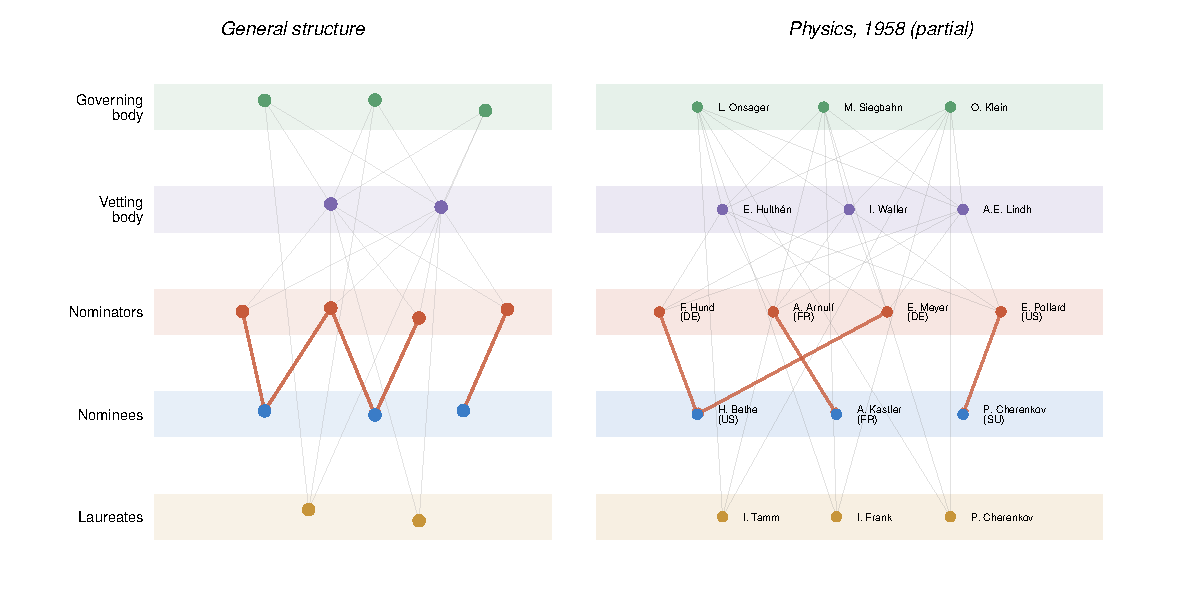
\includegraphics[width=\textwidth]{Figures/fig1_schematic.pdf}
\caption{\textbf{Multilayer network of the Nobel Prize selection process.} All edges are directed top to bottom. (\textbf{A})~General structure (illustrative): grey edges show dense institutional connections; terracotta edges show sparse, selective nomination decisions. The nominee--laureate visual connection illustrates the selection outcome; no nominee $\to$ laureate edge type is modeled. (\textbf{B})~Subset of the 1958 Physics network with real individuals, showing selected nodes and edges; the full network for this prize-year contains additional individuals. Country codes indicate professional country: DE, Germany; FR, France; SU, Soviet Union; US, United States.\label{fig:schematic}}
\end{figure}

% Figure 2: Edge-type homophily bars (generated by 12_figures.R)
\begin{figure}
\centering
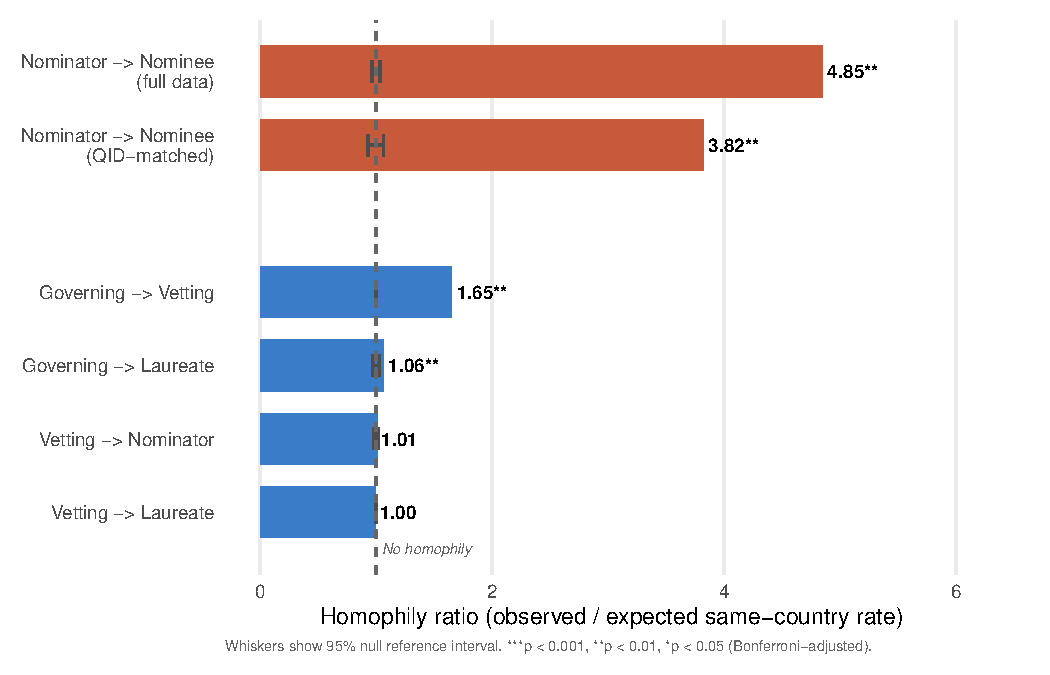
\includegraphics[width=\textwidth]{Figures/fig2_edge_homophily.pdf}
\caption{\textbf{Geographic homophily by edge type.} Country-level homophily ratios, defined as observed divided by expected same-country rate. Dashed line at 1.0: geographic neutrality. Terracotta: nomination edges; steel blue: institutional edges. Homophily concentrates at the nomination edge, at 4.85; institutional edges cluster near 1.0, as expected from the complete bipartite construction (see text).\label{fig:edge_homophily}}
\end{figure}

% Figure 3: Self-nomination heatmap (generated by 12_figures.R)
\begin{figure}
\centering
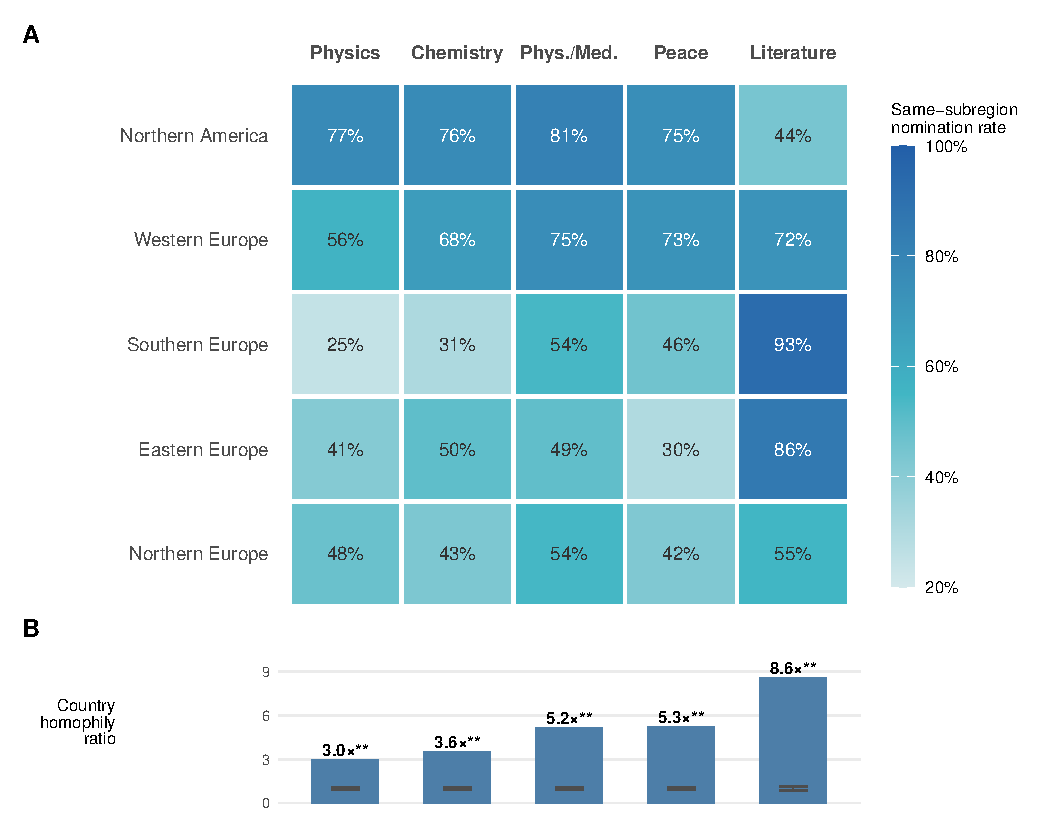
\includegraphics[width=\textwidth]{Figures/fig3_heatmap.pdf}
\caption{\textbf{Within-subregion nomination rates by prize and subregion.} (\textbf{A})~Percentage of nominations where nominator and nominee share the same subregion, with sample sizes in parentheses; white indicates low rates, dark blue high. (\textbf{B})~Country-level homophily ratios by prize.\label{fig:heatmap}}
\end{figure}

% Figure 4: Temporal paradox (generated by 12_figures.R)
\begin{figure}
\centering
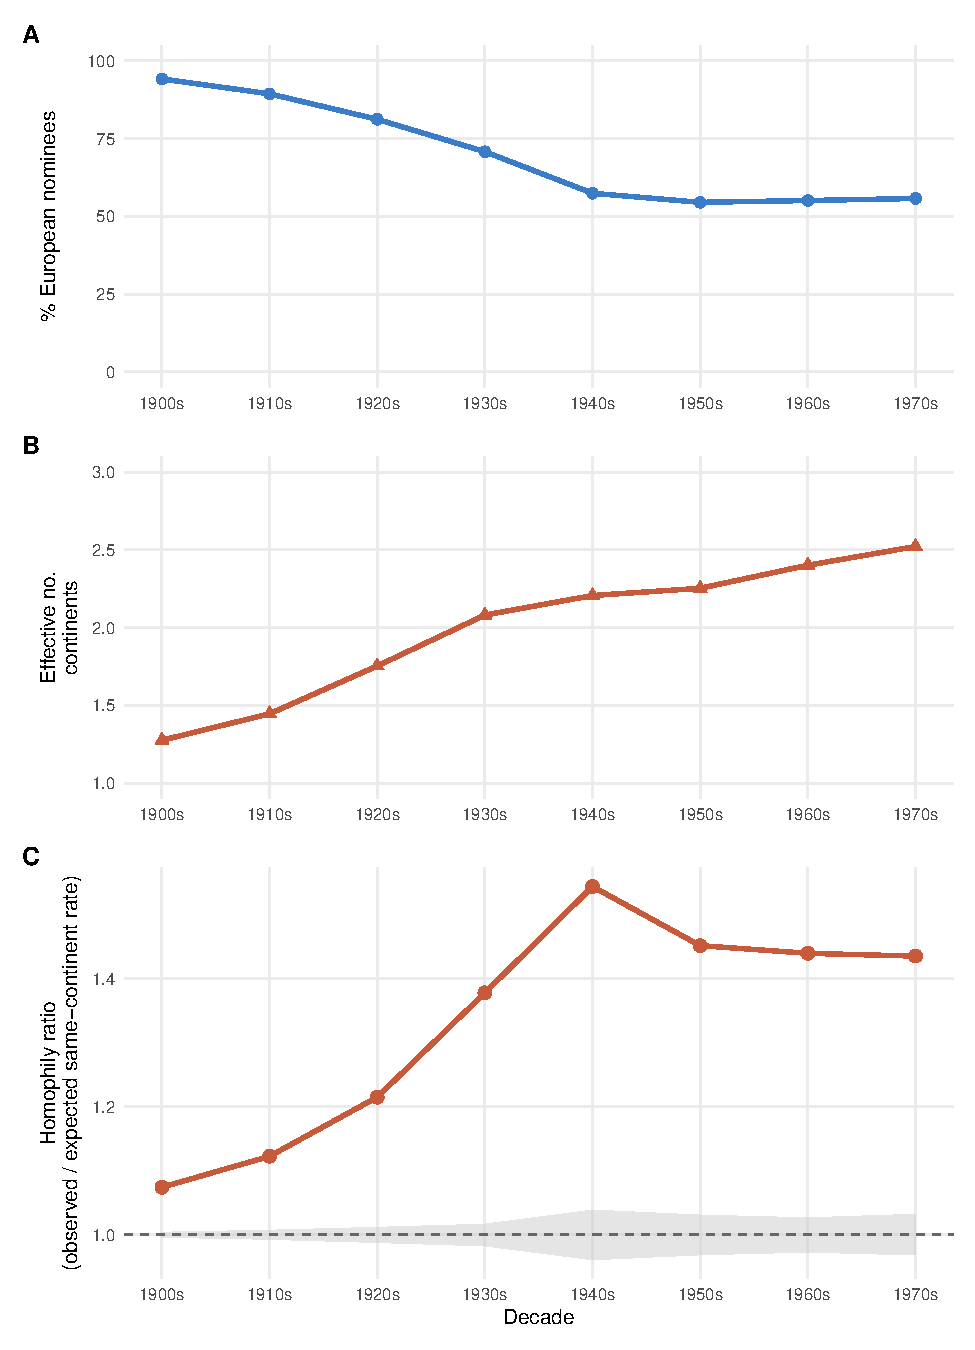
\includegraphics[width=\textwidth,height=0.75\textheight,keepaspectratio]{Figures/fig4_temporal.pdf}
\caption{\textbf{Temporal dynamics of pool diversification and nomination homophily.} (\textbf{A})~European nominee share declines over time. (\textbf{B})~Effective number of continents rises, indicating growing geographic diversity. (\textbf{C})~Continent-level homophily ratio over time with 95\% permutation reference interval (grey). The ratio rises despite diversification, partly reflecting ratio mechanics: the expected same-continent rate $E$ falls faster than the observed rate $O$. However, the raw difference $O - E$ also rose through the 1940s, confirming the increase is not purely mechanical (see text).\label{fig:temporal}}
\end{figure}

\clearpage

% =============================================
% SUPPLEMENTARY MATERIALS
% =============================================

% Reset counters for supplement
\setcounter{figure}{0}
\renewcommand{\thefigure}{S\arabic{figure}}
\setcounter{table}{0}
\renewcommand{\thetable}{S\arabic{table}}
\setcounter{equation}{0}
\renewcommand{\theequation}{S\arabic{equation}}

\begin{center}
{\large\textbf{Supplementary Materials for}}\\[6pt]
{\large\textbf{\scititle}}\\[12pt]
Chad M.\ Topaz$^{1,2,3,\ast}$,
Anvi Kurongonayini$^{2}$,
Bennett Ptak$^{2}$,
Arden Fluehr$^{2}$,
Ariana Mendible$^{4}$,
Rachel Roca$^{5}$,
Nancy Rodr\'{i}guez$^{3}$,
Lu Xian$^{6}$,
R\'{e}gan Schwartz$^{2}$,
Jude Higdon$^{1,7}$\\[6pt]
{\small $^{1}$QSIDE Institute.
$^{2}$Williams College.
$^{3}$University of Colorado--Boulder.
$^{4}$Seattle University.
$^{5}$Michigan State University.
$^{6}$University of Michigan.
$^{7}$Bennington College.}\\[4pt]
{\small $^\ast$Corresponding author. Email: cmt6@williams.edu}
\end{center}

\bigskip

\noindent This PDF file includes:
\begin{itemize}
\item Materials and Methods
\item Supplementary Text
\item Fig.\ S1
\item Tables S1 to S6
\end{itemize}

\clearpage

\subsection*{Materials and Methods}

\subsubsection*{Network Model}

We adopted a multilayer network framework \cite{Kivela2014} to represent the hierarchical Nobel Prize selection process. The full selection pipeline involves six categories of actors (Table~\ref{tab:selection_process} in the Supplementary Text); we retained five. We excluded potential vetters (impractical to enumerate for the Peace Prize, and identical to or a superset of the governing body for the other four prizes) and the selection body (identical to the governing body for four prizes, and to the vetting body for Peace). The five layers are: governing body, vetting body, nominators, nominees, and laureates. Our analysis examined each of the five directed edge types (enumerated in Network Construction below) independently rather than modeling inter-layer coupling; future work could use coupled multilayer null models to assess how homophily in one layer constrains outcomes in others.

Each unique individual occupies a single node carrying demographic attributes such as gender and nationality. Individuals may appear in multiple layers, across prizes, and across years. For example, Marie Curie was a Physics nominee (1902--1903), a Physics nominator (1905, 1910), and a Chemistry nominee and laureate (1911). Edges are directed and carry metadata: the two connected nodes, the year, the prize category, and the source and target layers. Thus, the directed edge from Gaston Darboux to Curie specifies 1911, Chemistry, and the nominator $\to$ nominee layer pair.

\subsubsection*{Data Acquisition}

No single source provides all data necessary for the network model. We gathered data for the five layers from multiple sources (Table~\ref{tab:data_sources}). While information about governing bodies, vetting bodies, and laureates is available through the present day, the Nobel Foundation's secrecy rule withholds nominator and nominee information until 50 years after the fact. All data were gathered programmatically in R using a reproducible pipeline of nine scripts, available in a public repository \cite{nobelgithub}. Below we describe each stage in sufficient detail for independent replication.

Assembling the data required two broad steps. First, we determined the identities of individuals in each network layer and when they served, using the sources in Table~\ref{tab:data_sources}. Second, we determined their demographic characteristics using Wikidata \cite{wikidata}, a structured open knowledge database that provides the structured data behind many Wikipedia pages. (For some bodies, such as the Swedish Academy and Storting, Wikidata serves as both roster and demographic source.) By using Wikidata, we relied on the choices its contributors made---for example, we used Wikidata's gender data rather than inferring gender ourselves, recognizing that demographic data not based on self-identification may be imperfect. Throughout the pipeline, we used Wikidata QIDs---unique entity identifiers of the form Q followed by a number---as the canonical identifier for each individual, enabling cross-referencing across data sources.

\begin{table}
\centering
\caption{\textbf{Sources for the data in each network layer.}}
\label{tab:data_sources}
\small
\begin{tabular}{lll}
\hline
\textbf{Network Layer(s)} & \textbf{Body} & \textbf{Source} \\
\hline
Governing Body/Selection Body & Royal Swedish Academy of Sciences & Swedish-language Wikipedia \\
& Karolinska Institutet & Project Runeberg \cite{KarolinskaEmployees} \\
& Swedish Academy & Wikidata SPARQL \cite{wikidata} \\
& Storting & Wikidata \cite{wikidata} \\
\\
Vetting Body & Nobel Committee for Chemistry & Wikipedia \cite{NobelCommitteeChemistry} \\
& Nobel Committee for Physics & Wikipedia \cite{NobelCommitteePhysics} \\
& Nobel Committee for Physio/Med & Wikipedia \cite{NobelCommitteePhysiology} \\
& Nobel Committee for Literature & the Swedish Academy website \cite{Ledamotsregister} \\
& Norwegian Nobel Committee & Wikipedia \cite{NorwegianNobelCommittee} \\
\\
Nominators & & the Nobel Prize website \cite{NobelPrizeWebsite} \\
\\
Nominees & & the Nobel Prize website \cite{NobelPrizeWebsite} \\
\\
Laureates & & Nobel Prize API v2.1 \\
\hline
\end{tabular}
\end{table}

\paragraph*{Governing Bodies.}

\emph{Royal Swedish Academy of Sciences (RSAS).} The RSAS awards the prizes in Physics and Chemistry. Members serve for life. We scraped the membership list from the Swedish-language Wikipedia page, which organizes members chronologically under bold year headers followed by bulleted lists of hyperlinked names. Founding members (1739) appear under the headings for founders and others. We parsed the rendered HTML by iterating through child elements in document order, updating the current induction year at each bold year header and extracting hyperlinked names from subsequent unordered lists, excluding redlinks and non-article links.

We resolved Wikidata QIDs in batch using the MediaWiki API, which maps up to 50 Wikipedia page titles to their corresponding Wikidata items per request and handles title normalization (e.g., converting underscores to spaces and resolving Unicode variants). We used exponential backoff (delay doubling from 2 seconds, up to 5 retries) for failed requests and a 0.2-second delay between batches. For each member, we recorded the induction year as the start year; end years were derived from Wikidata death dates (since membership is lifelong, the end of service coincides with death). Where multiple records existed for the same QID (e.g., due to class transfers within the Academy), we retained only the earliest induction record. The final dataset contains 2,312 RSAS members spanning 1739--2025, all with resolved QIDs.

\emph{Swedish Academy.} The Swedish Academy awards the Prize in Literature. Its 18 members serve for life. We queried Wikidata via SPARQL, selecting all individuals holding the position ``member of the Swedish Academy'' and excluding honorary members. Start and end dates were extracted from position qualifiers and parsed from Wikidata's ISO 8601 datetime format. All SPARQL queries throughout the pipeline were executed via HTTP POST to the Wikidata Query Service endpoint, with exponential backoff (5-second base delay, up to 10 retries) and a descriptive User-Agent string per Wikidata's access policy. The query yielded 202 member records.

\emph{Storting (Norwegian Parliament).} The Storting appoints the Norwegian Nobel Committee, which awards the Peace Prize. We queried Wikidata for all entities classified as human who hold the position ``member of the Storting'', extracting start and end dates from position qualifiers. Norwegian parliamentarians may serve non-consecutive terms; we consolidated overlapping terms by grouping each member's service periods chronologically and merging periods in which the gap between the end year of one term and the start year of the next was at most one year. We preserved non-consecutive terms as separate records. This yielded 4,281 member-term records spanning 1814--2025.

\emph{Karolinska Institutet.} The Karolinska Institutet (KI) awards the Prize in Physiology or Medicine. Before 1977, all KI full professors constituted the selection body; in 1977, the Nobel Assembly was established as a distinct entity, and in 1984 its membership was fixed at 50. Neither Wikidata nor KI's website publishes a complete roster of the Nobel Assembly.

We compiled KI professor data from Project Runeberg's digitized editions of the Swedish state calendar, covering 1881--1970. We manually mined fourteen editions for each professor's name, start year, and end year, then matched individuals to Wikidata QIDs, verifying that biographical information was consistent. We retained the 140 records with confirmed QIDs and both start and end years.

Post-1970 Nobel Assembly membership is not publicly available: Wikidata contains essentially no membership records for the Nobel Assembly, KI's website does not publish a roster, and Project Runeberg's digitized calendars stop circa 1972. This is a known structural gap (see Limitations).

\paragraph*{Vetting Bodies (Nobel Committees).}

Each prize has a dedicated Nobel Committee that reviews nominations and prepares recommendations for the governing body.

\emph{Chemistry, Physics, and Physiology/Medicine Committees.} These three committees are documented on Swedish-language Wikipedia. We extracted membership lists using a general-purpose parser that fetches wikitext via the MediaWiki API, splits text into sections by heading markers, and pulls bullet-list entries from sections for former members, current members, and secretaries. We parsed Wikipedia article titles from double-bracket link syntax, extracted start and end years via regular expressions, and resolved QIDs through the batch MediaWiki API. The Swedish Wikipedia page for the Physiology/Medicine committee explicitly states that the list is incomplete. Final counts: Chemistry 50 members, Physics 51, Physiology/Medicine 72 (59 with QIDs).

\emph{Literature Committee.} The Nobel Committee for Literature is drawn from the Swedish Academy. No standalone membership list exists on Wikipedia, so we extracted committee service years from individual member biographies on the Swedish Academy website. We queried Wikidata for all Swedish Academy members with their seat numbers and constructed biography page URLs following the site's convention.

The Swedish Academy website is a Nuxt.js single-page application. Rather than executing JavaScript, we extracted biography text directly from the embedded script tag in each page's HTML source, decoded HTML entities, stripped markup tags, and searched for mentions of Nobel Committee followed by year ranges. Two-digit years were expanded to four digits based on context. We retained only members whose biographies mentioned Nobel Committee service, yielding 35 members. This extraction method may break if the Swedish Academy redesigns its website.

\emph{Norwegian Nobel Committee.} The Norwegian Nobel Committee both vets nominations and awards the Peace Prize. We parsed the membership table from the English Wikipedia page, extracting start and end years and resolving QIDs via the batch MediaWiki API. This yielded 61 members (57 with QIDs).

\paragraph*{Nominations.}

We scraped the Nobel Prize Nomination Archive, which operates under a 50-year secrecy rule. As of 2025, records extend through 1974 or 1975 for Physics, Chemistry, Literature, and Peace. Physiology or Medicine nominations extend only through 1953; the Karolinska Institutet has not released records for 1954--1974, likely because of the 1977 Swedish transparency law and the concurrent restructuring that created the Nobel Assembly.

The archive's web interface uses numeric prize codes in its URL parameters (Physics = 1, Chemistry = 2, Physiology or Medicine = 3, Literature = 4, Peace = 5). For each of 353 prize-year combinations, we retrieved the list page and extracted all nomination IDs from links to detail pages. We then scraped each detail page to extract the nomination year, prize category, names, and internal person IDs of all nominees and nominators, and per-nomination contextual fields. Detail pages use a two-column table layout with bold section headers followed by labeled rows containing person links and metadata. For nominees, contextual fields include university, city, country, and (for some prizes) profession; for nominators, they include profession, university, city, and country. We parsed each detail page by iterating through table rows in document order, tracking the active section header and accumulating labeled fields for each person block. Country values were cleaned by stripping trailing ISO 3166 codes.

A single nomination may list multiple nominees (16.3\% of nominations) and, more rarely, multiple nominators (1.1\%), reflecting joint nominations and co-signed nomination letters; we generated all pairwise nominee--nominator combinations.

We standardized prize names to a common vocabulary and handled the Peace Prize archive's different header format as a special case. List pages were fetched sequentially with 0.5-second delays; detail pages were fetched in parallel across $N-1$ CPU cores (capped at 12) with 0.2-second per-worker delays and checkpointed after each prize-year. The final dataset contains 27,958 nomination records spanning 22,600 unique nominations, 4,006 unique nominees, and 11,650 unique nominators. Of these, 780 records (2.8\%) have anonymous or unlisted nominators, and 2 represent self-nominations.

\paragraph*{Laureates.}

We retrieved all Nobel Prize laureates from the official Nobel Prize API (v2.1), which provides structured JSON data including Wikidata QIDs, names, gender, award year, prize category, prize portion, motivation text, and primary affiliation at the time of award. We paginated through all results and filtered to the five original prize categories, excluding the Sveriges Riksbank Prize in Economic Sciences, established in 1969. Laureates who received multiple prizes appear as separate records per prize. The final dataset contains 927 laureate-prize records representing 919 unique individuals, with 100\% QID coverage.

\paragraph*{Entity Resolution for Nomination Archive People.}

The nomination archive identifies people by internal numeric IDs and names only, without Wikidata QIDs or other persistent identifiers. To integrate nomination data with the rest of the network, we developed a two-stage matching procedure.

In the first stage, for each of the 14,474 unique people in the nomination archive, we scraped their \emph{person} detail page on nobelprize.org (distinct from the nomination detail page), extracting last name, first name, gender, birth year, and death year from labeled table cells. Scraping was parallelized across available cores in chunks of 500 with disk checkpointing. Of the 14,474 people, 4,571 (31.6\%) had birth years recorded; the remaining 9,903 (68.4\%) lacked birth year data entirely. One birth-year record lacked a usable name, leaving 4,570 matchable individuals. Six records contained non-standard gender codes; we verified these individuals by first name, confirmed they are male, and recoded accordingly. One record had a transposed death year, corrected manually.

In the second stage, for each of the 4,570 matchable individuals, we implemented a three-phase Wikidata matching procedure. In Phase~1, we generated up to three name variants per person and searched the Wikidata entity search API in parallel, collecting all candidate QIDs. In Phase~2, we deduplicated candidates and batch-fetched their birth years from Wikidata via SPARQL in groups of 50, accepting a match only when a candidate's birth year exactly equaled the year in the Nobel archive. We prioritized precision over recall, with no fuzzy name or approximate year matching. In Phase~3, we exploited the nondeterministic ordering of Wikidata's search API: for still-unmatched individuals, we repeated the full-name search up to 100 additional times, as each query may surface different candidates. We cached birth year lookups from previous phases. Phase~3 terminated when no new matches were found or the maximum passes were reached.

This procedure matched 3,951 of 4,570 matchable individuals (86.5\%), representing 27.3\% of all nomination archive people. Among matched individuals, 44 had multiple Wikidata candidates with matching birth years; we retained the API's top-ranked candidate and recorded the multi-match count for potential manual review. An additional 619 matchable individuals (4.3\%) remained unmatched despite having birth year data, likely because their Wikidata entries use different name transliterations or do not appear among the API's top results. The remaining 9,904 people (68.5\%) lacked either birth year or name data, rendering Wikidata disambiguation infeasible. Unmatched individuals are represented using temporary identifiers with a \texttt{NOM:} prefix (e.g., \texttt{NOM:7283}), preserving the nomination-layer topology.

\paragraph*{Demographic Enrichment.}

We fetched demographic attributes from Wikidata for all individuals with resolved QIDs: English name label, gender, country of birth, nationality, birth date, death date, occupation, and employer/institution. Queries were executed in batches of up to 200 QIDs using the SPARQL \texttt{VALUES} clause, with individual fallback queries for failed batches. Multi-valued fields were collapsed into semicolon-delimited strings. Where multiple birth or death dates existed for a single QID, we retained the first non-missing value. After the initial fetch for governing body, vetting body, and laureate QIDs, we performed a second pass for the 3,951 matched nomination archive people, then re-collapsed all records to produce a single row per QID.

As a post-processing step, we derived end-of-service years for RSAS members from Wikidata death years, since lifelong membership means end of service coincides with death. Of 2,312 RSAS members, 1,871 received derived end years; 441 remained without (likely living members or individuals with unrecorded death dates). The final demographics table contains 10,206 unique individuals.

\paragraph*{Geographic Standardization.}

Country names originate from two sources with different conventions: Wikidata English labels (mixed case, including historical entities such as ``Austrian Empire,'' ``Kingdom of Prussia,'' and ``Russian Empire'') and the Nobel Prize nomination archive (uppercase modern and legacy names, sometimes annotated with ISO codes or legacy state names). We standardized all country names to modern sovereign states, United Nations M49 subregions (14 distinct values in our data), and continents (6 values) using a case-insensitive mapping table covering approximately 250 observed name variants.

We mapped historical entities to their most commonly associated modern successor state (e.g., the Austrian Empire and Austria-Hungary $\to$ Austria; Kingdom of Prussia and German Empire $\to$ Germany; Russian Empire and U.S.S.R.\ $\to$ Russia; Czechoslovakia $\to$ Czech Republic; Ceylon $\to$ Sri Lanka). These mappings are necessarily imperfect: the U.S.S.R.\ comprised 15 republics, and dissolved states such as Czechoslovakia and Yugoslavia had citizens from multiple successor nations. We assessed the impact of these recodings in the worst-case sensitivity analysis below. We pre-cleaned nomination archive country fields by stripping legacy annotations and flagging clearly invalid values (city names, institutional fragments) as missing, affecting approximately 0.9\% of records. For the demographics table, we added standardized columns for birth country, subregion, and continent; for the nominations table, analogous columns for both nominee and nominator. Multi-valued nationality fields were standardized entry by entry.

Mapping coverage was high: 100\% of non-missing birth country values in the demographics table, 99.9\% of nominee country values, and 99.7\% of nominator country values. The continental distribution is predominantly European (7,129 of 8,462 with non-missing birth country), followed by the Americas (975), Asia (245), Africa (60), and Oceania (53).

\subsubsection*{Network Construction}

We assembled the final network from all intermediate data files. Nodes correspond to unique individuals identified by Wikidata QIDs, with demographic attributes from the enrichment step. Edges are directed, carrying metadata for year, prize category, and source and target layers. We defined five edge types reflecting the institutional flow of the selection process:

\begin{enumerate}
    \item \textbf{Governing body $\to$ vetting body.} For each prize and calendar year from 1901 through 1975, we created edges from all active governing body members to all active vetting body members. A member is ``active'' in year $Y$ if their start year is at or before $Y$ and their end year (if known) is at or after $Y$. This complete bipartite construction captures the ongoing institutional oversight relationship, not just a snapshot at the moment a vetting member joins.

    \item \textbf{Vetting body $\to$ nominator.} For Chemistry, Physics, and Physiology/Medicine, Nobel Committees solicit nominations from qualified individuals. For each prize-year, we created edges from all active vetting body members to all nominators who submitted that year. Because the target set comprises nominators who actually submitted (not all who were invited), this edge type reflects the \emph{realized} pool rather than the underlying invitation list, which is unobserved. Any inference about invitation neutrality, therefore, assumes that response rates do not vary systematically by geography. Literature and Peace are excluded because their nomination processes are eligibility-based rather than purely invitation-based (Table~\ref{tab:selection_process}).

    \item \textbf{Nominator $\to$ nominee.} Direct edges from each nominator to each nominee within a nomination record. For nominations with multiple nominees or nominators, all pairwise combinations were generated and then deduplicated.

    \item \textbf{Governing body $\to$ laureate.} For Chemistry, Physics, Physiology/Medicine, and Literature, we created edges from all governing body members active in the award year to the laureate.

    \item \textbf{Vetting body $\to$ laureate.} For Peace only, the Norwegian Nobel Committee both evaluates nominations and awards the prize. Edges connect active committee members in the award year to the laureate.
\end{enumerate}

The body-to-prize mappings are: RSAS $\to$ \{Chemistry, Physics\}; Karolinska Institutet $\to$ Physiology/Medicine; Swedish Academy $\to$ Literature; Storting $\to$ Peace. Because the RSAS (founded 1739), Storting (founded 1814), and Swedish Academy (founded 1786) predate the Nobel Prize, we filtered governing body records to the Nobel era: members whose end-of-service year precedes 1901 were excluded. Members with unknown end years were retained under the assumption they may still have been active in 1901 or later.

After deduplication, the network contains 8,134 nodes (each a unique Wikidata QID; unmatched nomination archive individuals use \texttt{NOM:} prefix identifiers in the edge list but are not counted as nodes) and 514,111 edges. Edge counts by type: governing body $\to$ vetting body (252,476; 49.1\%), governing body $\to$ laureate (146,761; 28.5\%), vetting body $\to$ nominator (87,492; 17.0\%), nominator $\to$ nominee (26,654; 5.2\%), and vetting body $\to$ laureate (728; 0.1\%). Edge counts by prize: Physics (199,934), Chemistry (167,210), Physiology/Medicine (71,229), Peace (62,994), and Literature (12,744). The lower Physiology/Medicine counts reflect the Karolinska data gap post-1970 and the truncated nomination archive (through 1953 only); the lower Literature count reflects the smaller Swedish Academy membership (18 seats).

The network contains 1,374 self-loops from individuals occupying roles in multiple layers simultaneously (e.g., governing body members who are also laureates). We retained all self-loops as genuine structural features.

Temporal coverage varies by edge type. Governing body $\to$ vetting body: 1901--1975. Governing body $\to$ laureate: 1901--2025 (full institutional rosters). Vetting body $\to$ nominator: earliest nomination year through 1974--1975 (1953 for Physiology/Medicine). Nominator $\to$ nominee: 1901--1974/1975 (1901--1953 for Physiology/Medicine). Vetting body $\to$ laureate (Peace only): 1901--2025. Cross-edge-type homophily comparisons should be interpreted in light of these differing temporal windows.

\subsubsection*{Data Quality Assessment}

We conducted a 50-point diagnostic audit of all intermediate and output data files (Table~\ref{tab:diagnostics}). Below, we discuss findings by data source and assess the dataset's fitness for network analysis.

\begin{table}
\centering
\caption{\textbf{Summary of data quality diagnostics across all data sources.} Checks are classified as passed (no issues) or warning (expected structural limitation or quality note).}
\label{tab:diagnostics}
\small
\begin{tabular}{lcc}
\hline
\textbf{Category} & \textbf{Checks Passed} & \textbf{Warnings} \\
\hline
File integrity & 12/12 & 0 \\
Governing bodies & 6/8 & 2 \\
Vetting bodies & 5/7 & 2 \\
Nominations & 1/2 & 1 \\
Entity resolution & 3/4 & 1 \\
Laureates & 2/4 & 2 \\
Demographics & 2/3 & 1 \\
Geographic standardization & 4/4 & 0 \\
Network structure & 3/6 & 3 \\
\hline
\textbf{Total} & \textbf{38/50} & \textbf{12} \\
\hline
\end{tabular}
\end{table}

\paragraph*{Governing bodies.} All four governing bodies achieved 100\% QID resolution. All year values fall within plausible historical ranges (1700--2026). Three RSAS records have start year exceeding end year due to anomalous death-year imputation; these represent upstream Wikidata errors and are documented but not corrected. Of 2,312 RSAS members, 441 (19.1\%) remain without end years after imputation (likely living members or individuals with unrecorded death dates) and are treated as currently active for edge construction.

\paragraph*{Vetting bodies.} QID completeness ranges from 81.9\% (Physiology/Medicine, reflecting the acknowledged incompleteness of its Swedish Wikipedia source) to 100\% (Chemistry, Physics, Literature). We cross-validated committee members against their parent governing bodies: 42 of 45 Chemistry committee members and 44 of 50 Physics committee members appear in the RSAS roster. Only 23 of 52 Physiology/Medicine committee members with resolved QIDs whose service overlapped the Karolinska roster period, 1881--1970, appear in that roster; the remaining unmatched members likely held non-professorial roles or joined after the roster's coverage ended, as the full committee list extends to 2025.

\paragraph*{Nominations.} All five prize categories are represented with year ranges matching expectations. All 27,958 records have nominee person IDs; 780 (2.8\%) lack nominator person IDs (anonymous or unlisted nominators). Contextual field completeness from the nomination detail pages is as follows: nominee country 94.7\%, nominator country 97.7\%, nominee city 71.9\%, nominator city 78.4\%, nominee profession 73.6\%, nominator profession 76.8\%, nominee university 45.2\%, and nominator university 42.1\%.

\paragraph*{Entity resolution.} Of 14,474 unique people in the nomination archive, 3,951 (27.3\%) were matched to Wikidata QIDs. Among the 4,570 matchable individuals (those with both name and birth year), the match rate is 86.5\%. The primary bottleneck is missing biographical data: 9,904 people (68.4\%) lack birth years, making disambiguation infeasible. An additional 619 (4.3\%) had birth years but could not be matched, likely due to transliteration differences or absent Wikidata entries. Among matched individuals, 44 mapped to multiple candidates with matching birth years (we retained the top-ranked candidate), and 47 QIDs mapped to multiple person IDs in the archive (transliteration variants or duplicate source identifiers). As a consequence, 7.6\% of edge endpoints use unresolved \texttt{NOM:} prefix identifiers, and 14.6\% of edges involve at least one such identifier. These edges preserve nomination-layer topology but cannot be linked to individuals in other layers.

\paragraph*{Laureates.} All 927 laureate-prize records have QIDs (100\% coverage), and all 919 unique QIDs appear in the nodes file. Of these, 267 lack governing body $\to$ laureate edges: 139 Peace laureates (expected, since Peace uses the vetting $\to$ laureate pathway) and 128 Physiology/Medicine laureates awarded after 1970 (the Karolinska data gap).

\paragraph*{Demographics.} The demographics table contains 10,206 unique QIDs with no duplicates. Completeness rates are: name 99.7\%, gender 99.6\% (91.7\% male, 8.0\% female), birth country 82.9\%, nationality 96.9\%, birth year 99.6\%, death year 84.3\%, occupation 97.8\%, and institutional affiliation 44.9\%. No records have birth years exceeding death years, and 57 records with birth years before 1700 correspond to historically accurate early members of the RSAS (founded 1739) and Storting (founded 1814).

\paragraph*{Geographic standardization.} All four geographic mapping checks passed. Among 8,462 demographics records with non-missing birth country, 100\% were successfully mapped to modern countries, UN subregions, and continents. In the nominations table, 99.9\% of nominee country values (26,446 of 26,466) and 99.7\% of nominator country values (27,230 of 27,302) were mapped. The small number of unmapped nomination country values correspond to legacy annotations or data artifacts that could not be resolved to a modern country.

\paragraph*{Network structure.} No duplicate edges exist. The vertex set comprises 8,134 QID-resolved individuals; unresolved \texttt{NOM:} prefix identifiers appear as edge endpoints in the nomination layer but are not counted as nodes, meaning the network is not a standard $G = (V, E)$ graph. Among edges with resolved QIDs on both endpoints, 6,157 nodes are involved (mean degree 142.6, median 28, maximum 14,978). A total of 1,131 nodes (13.9\%) are isolates---individuals matched to QIDs whose nomination-layer edges still reference their \texttt{NOM:} identifiers, creating split representations. This identity-splitting does not affect primary homophily analyses: the nominator $\to$ nominee ratio is computed directly from per-nomination geographic fields (keyed to nomination records, not QIDs), and institutional-layer analyses use only QID-resolved edges. Isolate nodes are excluded from degree distributions.

\paragraph*{Known Structural Gaps.}

We document seven structural limitations inherent to the available sources:
\begin{enumerate}
    \item \emph{Karolinska Institutet post-1970 gap.} Nobel Assembly membership after 1970 is not publicly available, resulting in missing governing body $\to$ laureate and governing body $\to$ vetting body edges for Physiology/Medicine after 1970.

    \item \emph{Nomination archive 50-year secrecy rule.} Nomination data are available through 1974--1975 for most prizes, but only through 1953 for Physiology/Medicine.

    \item \emph{Physiology/Medicine vetting body incompleteness.} The Swedish Wikipedia source for this committee is self-reportedly incomplete.

    \item \emph{Literature committee extraction fragility.} Committee service years were parsed from a Nuxt.js SPA payload, which may break if the Swedish Academy redesigns its website.

    \item \emph{Nomination QID match rate.} While 86.5\% of matchable individuals (those with birth years) were resolved to Wikidata QIDs, only 27.3\% of all nomination archive people were matched, because 68.4\% lack birth years entirely.

    \item \emph{RSAS end-year imputation.} 19.1\% of RSAS members lack end years after death-year imputation and are treated as currently active, which may slightly overcount active members in recent years.

    \item \emph{Storting term consolidation.} Non-consecutive Storting terms are preserved, but gaps between terms may not perfectly reflect actual departure and return dates.
\end{enumerate}

\paragraph*{Fitness for Network Analysis.}

Despite these gaps, the dataset is suitable for multilayer network analysis. Governing body layers have 100\% QID resolution; vetting body resolution ranges from 81.9\% (Physiology/Medicine) to 100\% (Chemistry, Physics, Literature), with the Norwegian Nobel Committee at 93.4\%. The laureate layer has 100\% QID coverage (1901--2025). The nomination layer achieves 86.5\% entity resolution among matchable individuals and preserves the full nominator--nominee structure through \texttt{NOM:} identifiers; per-nomination contextual data---country (94.7--97.7\%), city (71.9--78.4\%), profession (73.6--76.8\%), university (42.1--45.2\%)---support geographic analyses even for individuals without resolved QIDs. The primary constraints are: (a)~Physiology/Medicine analyses are limited by the Karolinska gap and truncated nomination archive; (b)~cross-layer analyses are limited to the 27.3\% of nomination archive people with resolved QIDs; and (c)~the 13.9\% isolate rate is an artifact of identifier resolution, not true network structure.

\subsubsection*{Network Analysis}

Our analysis centered on geographic homophily: the tendency for connected individuals to share geographic origin more than expected by chance. We measured homophily at three nested scales---country, United Nations M49 subregion (14 categories), and continent (6 categories)---and decomposed it across the five edge types defined above.

\paragraph*{Network Descriptive Statistics.}

The full network comprises 8,134 nodes and 514,111 directed edges, yielding a density of 0.0078. Nomination edges (26,654) connect 11,642 unique nominators to 3,927 unique nominees (the archive lists 11,650 distinct person identifiers, but eight pairs resolve to the same Wikidata entity under variant name spellings). The median nominator out-degree is 1 (mean 2.3, max 94), reflecting that most nominators submit few nominations. The median nominee in-degree is 2 (mean 6.8, max 169), indicating that a small number of candidates attract many nominations while most receive few. Institutional edges (487,457) arise from complete bipartite expansion and thus have high degree counts that reflect layer sizes rather than individual-level connections.

\paragraph*{Homophily Ratio.}

For a given set of directed edges, let $f_i$ denote the fraction of source \emph{edge endpoints} from geographic category $i$ and $t_i$ the fraction of target endpoints from category $i$ (computed over the edge list, not unique nodes, so individuals contributing more edges receive proportionally more weight). Under independent pairing, the expected same-category rate is $E = \sum_i f_i \cdot t_i$. The observed rate $O$ is the fraction of edges whose source and target share a category. The \emph{homophily ratio} $H = O / E$ equals 1 under geographic neutrality; values above 1 indicate homophily, below 1 heterophily. As a complementary measure, we computed Newman's assortativity coefficient \cite{New2003} $r = \frac{\sum_i e_{ii} - \sum_i a_i b_i}{1 - \sum_i a_i b_i}$, where $e_{ii}$ is the fraction of edges connecting same-category nodes, and $a_i$ and $b_i$ are the fractions of edge endpoints originating from and terminating in category $i$. For the primary nominator $\to$ nominee edge at the country level, $r = 0.41$, confirming strong geographic sorting.

Geographic data comes from two sources. The nomination archive records country of professional activity at the time of each nomination (e.g., Enrico Fermi appears as ``Italy'' in 1935--1938 and ``United States'' post-1939). For all other edge types, geographic attributes come from Wikidata birth country. The primary nominator $\to$ nominee analysis therefore measures sorting by professional affiliation; institutional-layer analyses measure sorting by birth country.

For the nominator $\to$ nominee edge type, we computed homophily directly from the nomination archive (94.7--97.7\% geographic completeness), using all 25,844 edges with non-missing geography rather than restricting to the 8,119 with resolved QIDs on both endpoints. As a robustness check, we re-estimated homophily using birth country from Wikidata for the QID-matched subset (Table~S4). The vetting body $\to$ nominator analysis does \emph{not} use the full 87,492 complete bipartite edges. Instead, it restricts to edges where both endpoints have resolved QIDs and non-missing birth country, necessary because vetting body geography comes from Wikidata. This restriction also mitigates the tautological tendency of the full bipartite expansion to push $H$ toward 1.0, since within any single prize-year block the complete expansion mechanically produces $O \approx E$. Only Chemistry, Physics, and Physiology/Medicine contribute (Literature and Peace are excluded by construction). After QID and geography filters, $N = 25{,}811$ edges remain. This analysis uses birth country for \emph{both} endpoints, unlike the primary nominator $\to$ nominee analysis. The near-coincidence between this $N$ and the 25,844 nominator $\to$ nominee records is accidental; they derive from different data sources and filtering pipelines.

\paragraph*{Permutation Tests.}

We assessed statistical significance using permutation tests with $N = 10{,}000$ rewirings. For each edge set, we held the source node vector fixed and permuted the target vector, preserving edge count and marginal geographic distributions while breaking observed pairing. The primary tests (Table~\ref{tab:homophily_edge_type}) pool across prize-years, so the null preserves pooled marginals but does not block by prize or year. Prize-specific and decade-specific tests serve as stratified analyses confirming results hold within temporal and disciplinary strata. The $p$-value is $(k + 1) / (N + 1)$, where $k$ is the number of replicates with same-geography rate at least as large as observed. For some institutional edge types at the continent scale, one endpoint's distribution is extremely concentrated (e.g., vetting bodies nearly 100\% European), producing a near-degenerate null; these yield $p = 1.000$, indicating the observed rate is no higher than expected. We also reported 95\% null reference intervals on homophily ratios---these represent the distribution under the null hypothesis of geographic independence, not confidence intervals for the observed ratio.

Our analysis conducted 49 statistical tests under formal multiple-comparisons control: edge-type decomposition (13 tests: 6 edge types $\times$ 2 scales, plus 1 subregion-level test; Table~\ref{tab:homophily_edge_type}), prize-specific homophily (5 $\times$ 3 = 15 tests), harmonized 1901--1953 prize comparisons (5 tests), and temporal trends (8 decades $\times$ 2 scales = 16 tests). An additional 38 prize-by-decade tests (continent level only) are treated as exploratory and excluded from the 49-test count. The primary finding ($H = 4.85$, $p < 0.001$) survives Bonferroni correction ($\alpha_{\text{adjusted}} = 0.05/49 \approx 0.0010$). Secondary findings should be interpreted with caution, as some may reflect false discoveries. We chose $N = 10{,}000$ permutations because the minimum reportable $p$-value ($\approx 0.0001$) provides clearance above the Bonferroni threshold while keeping computation tractable. All tests were parallelized using the \texttt{furrr} package in R. The primary test does not condition on covariates such as discipline or institutional ties. We therefore also ran a blockwise permutation test that shuffles target geographies \emph{within} each prize-year block. Because $H$ is defined from pooled rates, it is invariant to the permutation scheme; only the $p$-value changes. The blockwise test yields $p < 0.001$ at all three scales, confirming the finding is not an artifact of aggregating heterogeneous blocks. Decade-stratified analyses (Table~\ref{tab:temporal_homophily}) show significant homophily within every decade, and prize-specific analyses show significant country-level homophily within every discipline (3.01--8.58), further ruling out aggregation artifacts.

\paragraph*{Clustered Permutation Test.}

Because the same nominators appear across multiple years, edges are not fully independent. To account for this, we conducted a clustered permutation test that shuffled geography labels at the nominator level rather than the edge level: each nominator's entire set of edges was reassigned to the geographic label of a randomly selected other nominator, preserving within-nominator correlation. With 10,000 permutations, the observed $H = 4.78$ (using the 25,363 edges with non-missing nominator ID and geography) far exceeds the 95\% null interval of [0.89, 1.05], yielding $p < 0.001$.

\paragraph*{Supra-Adjacency Assortativity.}

To characterize the system-wide geographic structure, we computed Newman's assortativity coefficient $r$ on the full supra-adjacency matrix (all edge types combined into a single directed graph), using birth country from Wikidata for all nodes to ensure a consistent geographic definition. At the country level, the full-network assortativity is $r = 0.19$, compared to $r = 0.26$ for nomination edges alone and $r = 0.19$ for institutional edges alone. The full-network value is pulled toward the institutional value because institutional edges outnumber nomination edges approximately 40:1. At the continent level, the contrast is sharper: nomination edges yield $r = 0.30$, institutional edges $r = 0.02$, and the full network $r = 0.03$. Individual institutional edge types show near-zero assortativity (governing body $\to$ laureate: $r = 0.003$; vetting body $\to$ nominator: $r = 0.001$; vetting body $\to$ laureate: $r = 0.000$), with the exception of governing body $\to$ vetting body ($r = 0.43$), which reflects the pooling of prize-awarding institutions: the RSAS serves both Chemistry and Physics, so pooling across these prizes inflates apparent same-country matching.

\paragraph*{Layer-Contrast Permutation Test.}

To formally test whether nomination-edge homophily exceeds institutional-edge homophily, we conducted a layer-contrast permutation test. Using birth country from Wikidata for all nodes (ensuring a consistent geographic definition across layers), we computed $\Delta H = H_{\text{nomination}} - H_{\text{institutional}}$ on the 328,721 edges with non-missing geography on both endpoints. For each of 10,000 permutations, we randomly reassigned the edge-type label (nomination vs.\ institutional) to each edge while preserving the total number in each class, then recomputed $\Delta H$. The observed $\Delta H = 2.37$ lies far outside the permutation null interval $[-0.04, 0.04]$ ($p < 0.001$), confirming that the between-layer contrast is not an artifact of differences in sample size or marginal distributions.

\paragraph*{Sensitivity to Prolific Nominators.}

Because multi-nominee and multi-nominator records are expanded to all pairwise combinations, and because some nominators participate across multiple years, prolific nominators could contribute a disproportionate share of edges. The expected rate ($E = \sum_i f_i \cdot t_i$) is based on marginal distributions of all endpoints, so heavy contributors influence both observed and expected rates. Nomination edges are deduplicated (identical nominator--nominee--year--prize tuples collapse to one edge), but the same dyad recurring in different years contributes one edge per year, representing distinct nomination decisions. The broad distribution of nominators (10,896 unique individuals across 25,844 geographically complete records) mitigates the influence of any single prolific nominator. A leave-out analysis confirms this: removing the top 1\% of nominators by edge count yields $H = 5.13$; top 5\%, $H = 5.34$; top 10\%, $H = 5.51$. The ratio \emph{increases} when prolific nominators are removed, indicating they are less homophilous than average and that the aggregate effect is distributed across many nominators.

\paragraph*{Worst-Case Bounds on Missing Data and Historical Recoding.}

We computed three worst-case sensitivity bounds on the primary finding ($H = 4.85$). \emph{Missing geography:} Of 27,958 records, 25,844 (92.4\%) have complete geography; 2,114 (7.6\%) are missing on at least one side. If all missing records were cross-country nominations, $H = 4.48$ (7.6\% reduction), still far above the permutation null upper bound ($\approx 1.10$). \emph{Historical country recoding:} Of 12,091 same-country edges, 432 (3.6\%) involve at least one historically recoded country. If all 432 were false matches, $H = 4.67$. \emph{Combined worst case:} Applying both adjustments simultaneously yields $H = 4.32$, still 4.3 times the expected rate under geographic independence.

\paragraph*{Diversity Metrics.}

To characterize layer composition, we computed the \emph{effective number of categories} as $\exp(-\sum_i p_i \log p_i)$, the exponential of Shannon entropy. This gives the equivalent number of equally represented categories: 1 indicates perfect concentration; higher values indicate greater diversity. At the country level, 84.7\% of governing body members and 96.3\% of vetting body members were born in Sweden, Norway, or Denmark, confirming the Scandinavian concentration of the institutional layers.

\paragraph*{Prize-Specific Temporal Tests.}

We repeated decade-by-decade permutation tests within each prize category separately (10,000 permutations per cell). All five prizes showed rising continent-level homophily: Chemistry 1.05 (1900s) to 1.53 (1970s); Physics 1.06 to 1.36; Physiology/Medicine 1.06 to 1.45 (through the 1950s); Literature 1.10 to 1.42; Peace 1.09 to 1.40. These results confirm the pattern is not an artifact of compositional shifts across categories. Note: these 38 tests are not subject to multiple-comparisons correction and should be interpreted with appropriate caution.

\paragraph*{Nomination Flow Asymmetry.}

To characterize directional asymmetry, we computed for each UN subregion the number of nominations sent (as nominator origin) and received (as nominee origin). The \emph{return ratio} is nominations received divided by sent. Ratios above 1 identify net importers of recognition; below 1, net exporters.

\paragraph*{Laureate Prediction Analysis.}

We tested whether same-country nominations are more likely to identify eventual laureates. Using the nomination archive with complete nominator and nominee geography, we computed for each nominee--prize pair the fraction of nominations received from same-country nominators. Nominees were classified as laureates or non-laureates by matching nominee QIDs to the laureate roster. At the nominee level, laureates received a lower mean fraction of same-country nominations (37.0\%) than non-laureates (52.7\%). To assess significance, we ran a permutation test (10,000 iterations) shuffling laureate labels among nominees; the observed difference exceeded all permuted values ($p < 0.001$). We also fit a logistic regression predicting laureate status from same-country nomination fraction, controlling for log total nomination count:
\[
\text{logit}(\Pr[\text{laureate}]) = \beta_0 + \beta_1 \cdot \text{same\_country\_frac} + \beta_2 \cdot \log(\text{total\_nominations}).
\]
The coefficient on same-country fraction was $\hat{\beta}_1 = -1.08$ (SE $= 0.14$, $z = -7.74$), corresponding to an odds ratio of 0.34; each unit increase in same-country nomination fraction is associated with a 66\% decrease in the odds of laureate status. The pattern holds within each of the five prize categories.

\paragraph*{Nominator Heterogeneity.}

To characterize individual variation in geographic homophily, we computed per-nominator same-country nomination rates for all nominators with at least two nominations in the archive (ensuring a non-degenerate rate). We compared Scandinavian nominators (those from Sweden, Norway, or Denmark) to non-Scandinavian nominators. Scandinavian nominators exhibited a mean same-country rate of 22.2\%, compared to 51.4\% for non-Scandinavian nominators. This finding provides individual-level confirmation that the institutional core of the Nobel system---housed in Scandinavia---is not the source of geographic sorting.

\paragraph*{Temporal Trend Tests.}

We tested the temporal trend in continent-level homophily using linear and piecewise regression on the eight decade-level homophily ratios from Table~\ref{tab:temporal_homophily}. A piecewise decomposition around the 1940s, motivated by the observed inflection at World War II, showed a statistically significant rise from the 1900s through the 1940s ($t = 7.84$) followed by a non-significant decline through the 1970s, consistent with a plateau. A full linear model over all decades showed a significant overall upward trend. These tests confirm that the temporal pattern described in the main text---rising homophily followed by persistence---is statistically robust.

\clearpage

\subsection*{Supplementary Text}

\subsubsection*{Nobel Prize Selection Process}

Nobel Prize selection processes are complex and opaque. No definitive scholarly source provides a complete description. We aim to fill this gap, drawing from the Nobel Prize website \cite{NobelPrizeWebsiteFull}, the Royal Swedish Academy of Sciences website \cite{RSAS}, the Karolinska Institutet website \cite{KINA}, and the Wikipedia entry for the Nobel Peace Prize \cite{NPPWiki}.

Table~\ref{tab:selection_process} summarizes the relevant actors for each prize. We focus on individuals who wield influence on the process and therefore exclude nominees and laureates. We begin with a general overview and then discuss each prize's specific features.

\begin{table}
\centering
\caption{\textbf{Overview of the process for selection of Nobel Laureates.} For each Nobel Prize, a governing body chooses from among a group of potential vetters in order to create a vetting body. The vetting body receives nominations made by nominators and creates a short list of viable laureates. The selection body takes the vetting body's input and makes the final choice of laureate.}
\label{tab:selection_process}
\small
\begin{tabular}{p{0.11\textwidth}p{0.14\textwidth}p{0.14\textwidth}p{0.14\textwidth}p{0.14\textwidth}p{0.14\textwidth}}
\hline
& \textbf{Chemistry} & \textbf{Physics} & \textbf{Physio/Med} & \textbf{Literature} & \textbf{Peace} \\
\hline
\textbf{Governing Body} & Royal Swedish Academy of Sciences & Royal Swedish Academy of Sciences & Nobel Assembly at Karolinska Institutet & Swedish Academy & Storting$^{a}$ \\
\hline
\textbf{Potential Vetters} & Royal Swedish Academy of Sciences & Royal Swedish Academy of Sciences & Karolinska Institutet & Swedish Academy & Norwegian politicians$^{b}$ \\
\hline
\textbf{Vetting Body} & Nobel Committee for Chemistry$^{c}$ & Nobel Committee for Physics$^{c}$ & Nobel Committee for Physio/Med & Nobel Committee for Literature$^{c}$ & Norwegian Nobel Committee \\
\hline
\textbf{Nominators} & By invitation based on stated eligibility criteria & By invitation based on stated eligibility criteria & By invitation based on stated eligibility criteria & Based on stated eligibility criteria$^{d}$ & Based on stated eligibility criteria \\
\hline
\textbf{Selection Body} & Royal Swedish Academy of Sciences & Royal Swedish Academy of Sciences & Nobel Assembly at Karolinska Institutet & Swedish Academy & Norwegian Nobel Committee \\
\hline
\end{tabular}

\smallskip
{\noindent\scriptsize\linespread{1.0}\selectfont
$^{a}$~The Storting is the Norwegian parliament.
$^{b}$~It is not a formal eligibility requirement to be a politician, nor to be Norwegian. However, the Storting has stated that ``As far as possible, the composition of the Committee is to reflect the relative strengths of the political parties in the Storting.'' Moreover, historically, all members of the committee have indeed been Norwegian.
$^{c}$~Five members of the Vetting Body are chosen by the Governing Body, and then several additional members of the Vetting Body are added by the Vetting Body itself; these are called \emph{co-opted} members.
$^{d}$~Similar to the Vetting Bodies for Chemistry, Physics, and Physiology/Medicine, the Vetting Body for Literature does send out letters soliciting nominations. However, unlike for those other prizes, for the Literature prize, individuals who meet certain eligibility requirements can nominate even if they did not receive a letter of invitation to do so.
\par}
\end{table}

Each prize has a \emph{governing body} that oversees the process. The governing body chooses from among \emph{potential vetters} to create a \emph{vetting body}, which solicits and/or receives nominations. For three of the five prizes, individuals can become \emph{nominators} only by invitation of the vetting body; for the other two, any eligible individual can nominate. After receiving nominations, the vetting body sends nominee portfolios to external experts for evaluation, assesses the nominees, and proposes a shortlist to the governing body, which makes the final selection.

The Chemistry and Physics prizes have the most similar processes. The governing body for both is the Royal Swedish Academy of Sciences (RSAS), established in 1739, with about 480 Swedish and 175 foreign members divided into ten classes. The Nobel Committees for Chemistry and Physics, each comprising five voting members from the relevant RSAS class, serve as vetting bodies. Each committee solicits nominations from qualified individuals (typically receiving 250--300), commissions external evaluations, and prepares a finalist report. The full RSAS then discusses and votes on the finalists, selecting one to three laureates per prize per year.

The Physiology or Medicine prize involves different actors. The governing body is the Nobel Assembly at the Karolinska Institutet, a medical research institute in Sweden; since 1984, the Assembly comprises 50 KI members. The vetting body is the Nobel Committee for Physiology or Medicine (five voting members appointed by the Assembly). The Assembly also serves as the selection body.

The Literature prize is governed by the Swedish Academy (not the RSAS), which has 18 members appointed for life. The Nobel Committee for Literature, selected from Academy members for three-year terms, serves as the vetting body. While the Committee solicits nominations, \emph{anyone} meeting the eligibility criteria may nominate. The Academy selects the laureate from the Committee's finalist list.

For the Peace Prize, the \emph{Storting} (Norwegian parliament) is the governing body. The Storting elects members of the Norwegian Nobel Committee for six-year terms. Unlike the science prizes, the Committee does not solicit nominations; as with Literature, anyone meeting eligibility criteria can nominate. The distinguishing feature is the complete \emph{absence of solicitation}, not the openness of eligibility (shared with Literature). Uniquely among the prizes, the selection body is the Norwegian Nobel Committee itself, not the governing body.

\clearpage

%%%%%%%%%%%%%%%% SUPPLEMENTARY FIGURE %%%%%%%%%%%%%%%

\begin{figure}
\centering
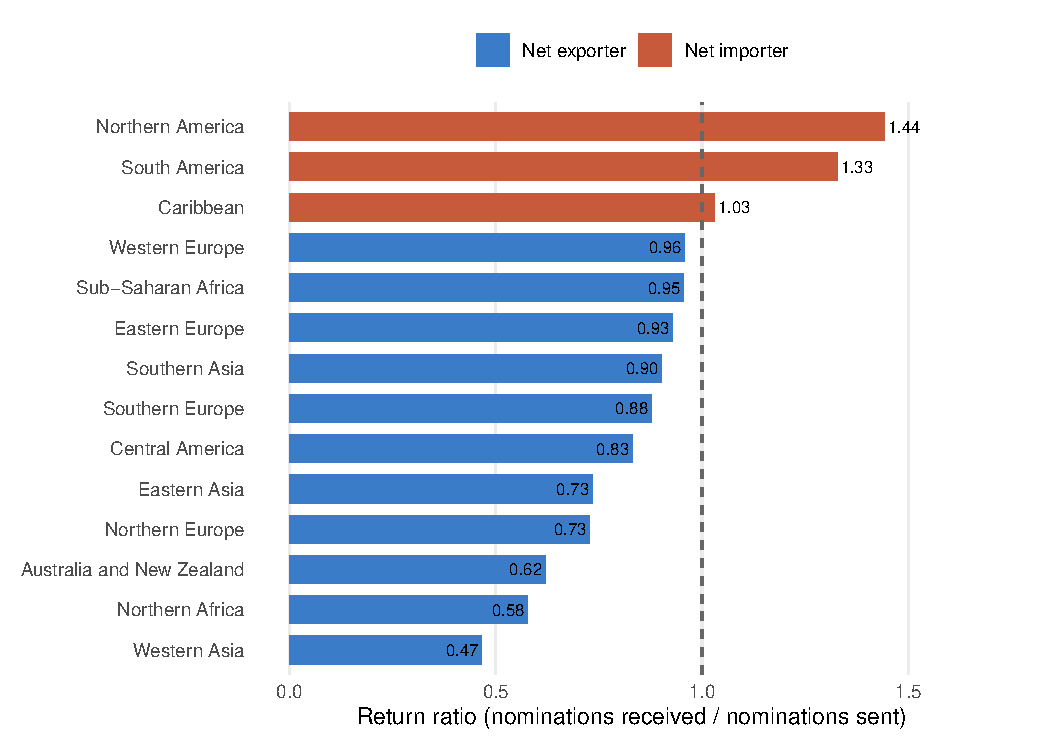
\includegraphics[width=\textwidth]{Figures/figS1_flow_asymmetry.pdf}
\caption{\textbf{Return ratios (nominations received / nominations sent) by UN subregion.} Terracotta bars indicate net importers of recognition (ratio $> 1$); steel blue bars indicate net exporters. Northern America is the largest net importer by nomination volume; Northern Europe, which houses the Nobel Prize institutions, is the largest net exporter by volume.\label{fig:flow}}
\end{figure}

\clearpage

%%%%%%%%%%%%%%%% SUPPLEMENTARY TABLES %%%%%%%%%%%%%%%

\begin{table}
\centering
\caption{\textbf{Geographic homophily by edge type and geographic scale.} The homophily ratio equals the observed same-geography rate divided by the expected rate under random pairing. $p$-values from 10,000 permutations.}
\label{tab:homophily_edge_type}
\footnotesize
\begin{tabular}{llrrrrc}
\hline
Edge type & Scale & $N$ & Obs. & Exp. & Ratio & $p$ \\
\hline
Nominator $\rightarrow$ Nominee & continent & 25,844 & 79.3\% & 58.0\% & 1.37 & $<$0.001 \\
Nominator $\rightarrow$ Nominee (QID subset) & continent & 8,119 & 74.0\% & 62.7\% & 1.18 & $<$0.001 \\
Governing $\rightarrow$ Laureate & continent & 96,506 & 50.6\% & 50.3\% & 1.01 & $<$0.001 \\
Governing $\rightarrow$ Vetting & continent & 197,756 & 94.5\% & 94.5\% & 1.00 & 1.000 \\
Vetting $\rightarrow$ Nominator & continent & 25,811 & 78.4\% & 78.4\% & 1.00 & 1.000 \\
Vetting $\rightarrow$ Laureate & continent & 529 & 48.6\% & 48.6\% & 1.00 & 1.000 \\
Nominator $\rightarrow$ Nominee & country & 25,844 & 46.8\% & 9.6\% & 4.85 & $<$0.001 \\
Nominator $\rightarrow$ Nominee (QID subset) & country & 8,119 & 32.1\% & 8.4\% & 3.82 & $<$0.001 \\
Governing $\rightarrow$ Vetting & country & 197,756 & 65.5\% & 39.7\% & 1.65 & $<$0.001 \\
Governing $\rightarrow$ Laureate & country & 96,506 & 4.4\% & 4.2\% & 1.06 & $<$0.001 \\
Vetting $\rightarrow$ Nominator & country & 25,811 & 5.5\% & 5.4\% & 1.01 & 0.069 \\
Vetting $\rightarrow$ Laureate & country & 529 & 1.7\% & 1.7\% & 1.00 & 1.000 \\
Nominator $\rightarrow$ Nominee & subregion & 25,844 & 60.8\% & 24.9\% & 2.44 & $<$0.001 \\
\hline
\end{tabular}
\end{table}

\begin{table}
\centering
\caption{\textbf{Temporal trends in nominee pool diversity and nomination homophily.} Homophily ratio measures continent-level geographic matching relative to the random expectation. $O - E$ is the raw difference between observed and expected same-continent rates, in percentage points. $p$-values from 10,000 permutations.}
\label{tab:temporal_homophily}
\small
\begin{tabular}{lrrrrrrrc}
\hline
Decade & $N$ & \% Eur. & Eff. cont. & Obs. & Exp. & $O - E$ & Ratio & $p$ \\
\hline
1900s & 2,825 & 94.2 & 1.28 & 95.6\% & 89.0\% & 6.6 & 1.07 & $<$0.001 \\
1910s & 2,634 & 89.4 & 1.45 & 92.8\% & 82.6\% & 10.1 & 1.12 & $<$0.001 \\
1920s & 3,193 & 81.2 & 1.75 & 88.1\% & 72.5\% & 15.6 & 1.21 & $<$0.001 \\
1930s & 4,206 & 70.8 & 2.08 & 82.1\% & 59.6\% & 22.5 & 1.38 & $<$0.001 \\
1940s & 2,151 & 57.4 & 2.21 & 76.7\% & 49.7\% & 27.0 & 1.54 & $<$0.001 \\
1950s & 3,178 & 54.5 & 2.25 & 70.6\% & 48.7\% & 22.0 & 1.45 & $<$0.001 \\
1960s & 4,417 & 55.1 & 2.40 & 69.4\% & 48.2\% & 21.2 & 1.44 & $<$0.001 \\
1970s & 3,240 & 55.7 & 2.52 & 65.6\% & 45.7\% & 19.9 & 1.43 & $<$0.001 \\
\hline
\end{tabular}
\end{table}

\begin{table}
\centering
\caption{\textbf{Demographic composition of each layer in the Nobel Prize multilayer network.} $N$ counts member-term records (an individual serving multiple non-consecutive terms contributes multiple records); for governing bodies, this principally affects the Storting. Governing body and vetting body counts reflect the full collected institutional rosters (extending beyond the 1901--1975 nomination window), because these bodies predate and postdate the archival period; nominator and nominee counts reflect the nomination archive window. Effective continents and subregions are computed as the exponential of Shannon entropy; a value of 1.0 indicates concentration in a single category, with higher values indicating greater geographic spread.}
\label{tab:layer_composition}
\small
\begin{tabular}{lrrrrr}
\hline
Layer & $N$ & \% Female & \% Europe & Eff. cont. & Eff. sub. \\
\hline
Governing bodies & 6,935 & 9.3 & 97.6 & 1.14 & 1.65 \\
Vetting bodies & 252 & 11.1 & 98.9 & 1.06 & 1.23 \\
Nominators & 11,650 & 2.3 & 71.3 & 2.24 & 6.30 \\
Nominees & 4,006 & 4.7 & 65.7 & 2.30 & 5.80 \\
Laureates (1901--1975) & 452 & 3.4 & 70.2 & 2.29 & 5.97 \\
\hline
\end{tabular}
\end{table}

\bibliographystyle{sciencemag}
\bibliography{bibliography}

\end{document}
